%%%%%%%%%%%%%%%%%%%%%%%%%%%%
% Do Elections Affect Fed Forecasts?
% Cassandra Grafström and Christopher Gandrud
%%%%%%%%%%%%%%%%%%%%%%%%%%%%

% !Rnw weave = knitr

\documentclass[a4paper]{article}\usepackage{graphicx, color}
%% maxwidth is the original width if it is less than linewidth
%% otherwise use linewidth (to make sure the graphics do not exceed the margin)
\makeatletter
\def\maxwidth{ %
  \ifdim\Gin@nat@width>\linewidth
    \linewidth
  \else
    \Gin@nat@width
  \fi
}
\makeatother

\IfFileExists{upquote.sty}{\usepackage{upquote}}{}
\definecolor{fgcolor}{rgb}{0.2, 0.2, 0.2}
\newcommand{\hlnumber}[1]{\textcolor[rgb]{0,0,0}{#1}}%
\newcommand{\hlfunctioncall}[1]{\textcolor[rgb]{0.501960784313725,0,0.329411764705882}{\textbf{#1}}}%
\newcommand{\hlstring}[1]{\textcolor[rgb]{0.6,0.6,1}{#1}}%
\newcommand{\hlkeyword}[1]{\textcolor[rgb]{0,0,0}{\textbf{#1}}}%
\newcommand{\hlargument}[1]{\textcolor[rgb]{0.690196078431373,0.250980392156863,0.0196078431372549}{#1}}%
\newcommand{\hlcomment}[1]{\textcolor[rgb]{0.180392156862745,0.6,0.341176470588235}{#1}}%
\newcommand{\hlroxygencomment}[1]{\textcolor[rgb]{0.43921568627451,0.47843137254902,0.701960784313725}{#1}}%
\newcommand{\hlformalargs}[1]{\textcolor[rgb]{0.690196078431373,0.250980392156863,0.0196078431372549}{#1}}%
\newcommand{\hleqformalargs}[1]{\textcolor[rgb]{0.690196078431373,0.250980392156863,0.0196078431372549}{#1}}%
\newcommand{\hlassignement}[1]{\textcolor[rgb]{0,0,0}{\textbf{#1}}}%
\newcommand{\hlpackage}[1]{\textcolor[rgb]{0.588235294117647,0.709803921568627,0.145098039215686}{#1}}%
\newcommand{\hlslot}[1]{\textit{#1}}%
\newcommand{\hlsymbol}[1]{\textcolor[rgb]{0,0,0}{#1}}%
\newcommand{\hlprompt}[1]{\textcolor[rgb]{0.2,0.2,0.2}{#1}}%

\usepackage{framed}
\makeatletter
\newenvironment{kframe}{%
 \def\at@end@of@kframe{}%
 \ifinner\ifhmode%
  \def\at@end@of@kframe{\end{minipage}}%
  \begin{minipage}{\columnwidth}%
 \fi\fi%
 \def\FrameCommand##1{\hskip\@totalleftmargin \hskip-\fboxsep
 \colorbox{shadecolor}{##1}\hskip-\fboxsep
     % There is no \\@totalrightmargin, so:
     \hskip-\linewidth \hskip-\@totalleftmargin \hskip\columnwidth}%
 \MakeFramed {\advance\hsize-\width
   \@totalleftmargin\z@ \linewidth\hsize
   \@setminipage}}%
 {\par\unskip\endMakeFramed%
 \at@end@of@kframe}
\makeatother

\definecolor{shadecolor}{rgb}{.97, .97, .97}
\definecolor{messagecolor}{rgb}{0, 0, 0}
\definecolor{warningcolor}{rgb}{1, 0, 1}
\definecolor{errorcolor}{rgb}{1, 0, 0}
\newenvironment{knitrout}{}{} % an empty environment to be redefined in TeX

\usepackage{alltt}
\usepackage{fullpage}
\usepackage[authoryear]{natbib}
\usepackage{setspace}
    \doublespacing
\usepackage{hyperref}
\hypersetup{
    colorlinks,
    citecolor=black,
    filecolor=black,
    linkcolor=cyan,
    urlcolor=cyan
}
\usepackage{dcolumn}
\usepackage{booktabs}
\usepackage{url}
\usepackage{tikz}
\usepackage[utf8]{inputenc} 

%%%%%%% Title Page %%%%%%%%%%%%%%%%%%%%%%%%%%%%%%%%%%%%%%%%%%%%
\title{Does Partisanship Affect Fed Inflation Forecasts?}

\author{Christopher Gandrud and Cassandra Grafstr\"{o}m}

\begin{document}


\maketitle

%%%%%%% Abstract %%%%%%%%%%%%%%%%%%%%%%%%%%%%%%%%%%%%%%%%%%%%
\begin{abstract}
\noindent\emph{Very Early draft version. Comments welcome.}\footnote{The paper is written with {\tt{knitr}} \citep{knitr2012} and is fully reproducible. Please contact us for the replication files.} \\[0.2cm]
Recent work argues that the Federal Reserve is not politically indifferent \citep{Clark2011}. The Fed tends to choose looser monetary policies during Republican administrations, possibly in order to ensure the (re)election of ideologically preferred administrations. This model excludes an essential aspect of monetary policy decision-making: expectations about future inflation. We use the Fed's Green Book forecasts and presidential election polling data to test whether expected electoral outcomes shape the estimates of future economic performance that influence FOMC policies. We find that Federal Reserve staff probably do not bias their forecasts to influence Fed governors around elections. However, they do systematically overestimate inflation during Democratic presidencies and underestimate inflation during Republican ones. This suggests that while not electorally motivated, Fed staff have a partisan bias when making inflation forecasts.

\end{abstract}

\begin{description}
  \item [{\textbf{Keywords:}}] forecast bias, Federal Reserve, rational partisan cycle,
\end{description}

\vspace{0.3cm}

Recent work argues that the Federal Reserve is not politically indifferent \citep{Clark2011}. The Fed tends to choose looser monetary policies during Republican administrations, possibly in order to ensure the (re)election of ideologically preferred administrations. This bias is assumed by Clark and Arel-Bundock to arise from a Board of Governors that prefer rightist presidents to leftist ones and so set interest rates to help Republican incumbents and hinder Democratic ones. 

Does this partisan preference also affect Federal Reserve staff's forecasts, which in turn influences Governors' interest rate decisions? 

An alternative possibility is that Federal Reserve staff may believe that inflation will be much higher under Democratic presidents. Employees within the Federal Reserve Banks may expect that Democratic presidents produce policies that increase inflation and Republican presidents produce policies that limit inflation. However, Republican and Democratic administrations both engage in largely expansionary fiscal policies. We argue that this leads to large overestimations of inflation during Democratic presidencies and a significant underestimation of inflation during Republican ones.

%THOUGHTS: THE DIFFERENCE IN ERRORS IMPLIES SOME SORT OF NAIVITE ON THE PART OF THE FED FORECASTERS IF THEY ALWAY THINK THAT THE REPUBLICAN PRESIDENT WILL SIGNIFICANTLY REDUCE SPENDING GROWTH AND FAILS TO WHILE THE DEMOCRATIC PRESIDENTS WILL SIGNIFICANTLY INCREASE SPENDING GROWTH AND FAIL TO. MAYBE THEY THINK THAT THE REPUBLICANS WILL ENGAGE IN POLICIES THAT LEAD TO HIGHER REAL GROWTH THROUGH THEIR TAX CUTS WHILE THE DEMOCRATS WILL ENGAGE IN PURELY SPENDING INCREASES (OR WITH TAX INCREASES) 

%CHRISTOPHER: HAVE WE TESTED TO SEE IF INFLATION IS ACTUALLY HIGHER UNDER DEMOCRATIC PRESIDENTS (ESPECIALLY AT THE ENDS OF THEIR TERMS) THAN IT IS UNDER REPUBLICAN PRESIDENTS? SINCE I BASICALLY HAVEN'T TOUCHED THE DATA I CAN'T REMEMBER. IF IT IS THEN THIS WOULD BE A NICE THING TO KNOW. IF THEY ARE ABOUT THE SAME THEN WE ARE BASICALLY SAYING THAT ECONOMISTS IN THE FED ARE NOT UPDATING (AND THIS IS IN LINE WITH BILL AND VINCENT'S ARGUMENT), WHEREAS IF THEY DIFFER THEN THEY ARE SIMPLY OVERSHOOTING BUT AREN'T NECESSARILY WRONG ON THE BASIC PREMISE.

In this paper we first provide a brief discussion of what Green Book inflation forecasts and forecast errors are, including their importance for monetary policy making and our current understanding of how they are made. As we demonstrate in this first section, academic scholarship up till now has not examined possible partisan causes of forecast erros. We then introduce the issues of inflation forecast partisan biases and posit a number of ways that Green Book forecasting may be influenced by them. We test these theories with a series of regression models using both unmatched and matched data on Green Book inflation forecast errors from the 1970s through 2005. The models suggest that, even when controlling for a number of important economic and political factors, Green Book forecasts show a distinct presidential partisan bias. 

%%%%%%%%%%%%%% Section 1: Forecasting Inflation at the Fed %%%%%%%%%%%%%%%%%%%%%

\section{Forecasting Inflation at the Fed \& Inflation Forecast Errors}

In this section we briefly describe what Green Book inflation forecasts and forecast errors are, why they are an important part of monetary policymaking in the United States, and the current understanding of how Federal Reserve inflation forecasts were made since the late 1960s.

\subsection{Forecasting \& Forecasting Errors}

Federal Reserve staff create ``Green Book" forecasts\footnote{Green Book data can be found at {\url{http://www.phil.frb.org/research-and-data/real-time-center/greenbook-data/philadelphia-data-set.cfm}}. Accessed December 2011.} before each meeting of the Federal Open Markets Committee (FOMC), the Federal Reserve's primary decision-making body. We focus on GNP/GDP price index forecasts.\footnote{Note: GNP was used to 1991 (inclusive) and GDP was used from 1992. Furthermore, the implicit deflator was used before the second quarter of 1996 and chain-weighted price index was used from the second quarter of 1996 onwards.} Green Book forecasts are made available for each quarter from the fourth quarter of 1964 through the end of 2005\footnote{There is a five year lagged release schedule}. We have 161 forecast quarters in our data set. Forecasts correspond to the FOMC meeting closest to the middle of the quarter. For a given quarter the data includes forecasts made in the present quarter and up to 5 quarters before. Actual inflation corresponding to each of these quarters\footnote{Inflation was calculated by comparing quarters year-on-year.} was found using data from the Federal Reserve Economic Data website.\footnote{\url{http://research.stlouisfed.org/fred2/}} Indicators comparable to the forecasted quantity are used, e.g. from the second quarter of 1996 we use the chain-weighted GDP price index. Absolute actual inflation for each quarter and inflation forecasts made two quarters before are compared in Figure \ref{absolute}. In general we use forecasts made two quarters before.\footnote{Using these two quarter forecasts constricts our observations so to 150 since, apart from the first quater of 1968, they are not included in the Green Book data before the fourth quarter of 1968.} 

%%%%%%%%%%%%%%%%%%%%%%%%%%  Raw Green Book estimate vs. actual graph
\begin{figure}[t]
    \caption{Green Book Inflation Forecasts and Actual Quarterly Inflation}
    \label{absolute}
    \begin{center}
    
\begin{knitrout}
\definecolor{shadecolor}{rgb}{0.969, 0.969, 0.969}\color{fgcolor}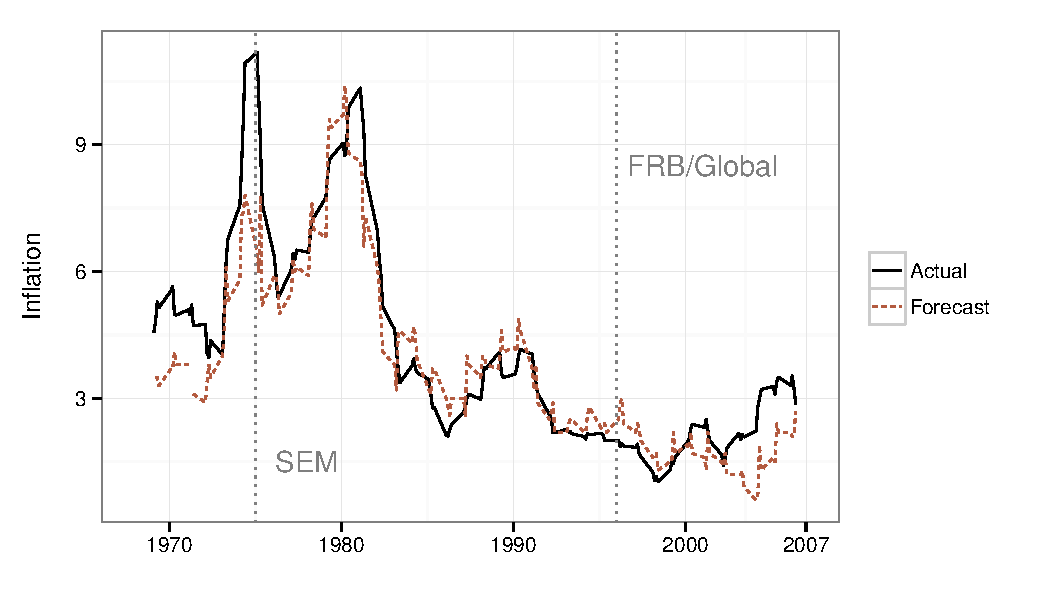
\includegraphics[width=0.8\linewidth]{figure/BaseInflation} 
\end{knitrout}

    
    \end{center}
    \begin{singlespace}
        {\scriptsize{Forecasts were made two quarters beforehand. \\
                     The grey dotted lines indicate the {\emph{approximate}} years that the Simultaneous Equation Models (SEM) and Federal Reserve Board Global (FRB/Global) forecasting models were fully implemented.  
                      }}
    \end{singlespace}
\end{figure}

We calculate {\bf{forecast error}} $E$ as the difference between the Green Book inflation forecast $F$ for a given quarter $q$ and actual inflation $I$ as a proportion of actual inflation
%
\begin{equation}
    E_{q} = \frac{F_{q} - I_{q}}{I_{q}}
\end{equation}
%
We put the error in terms of actual inflation to control for the fact that mean actual inflation varies considerably across different periods (see Figure \ref{absolute}). 

\subsection{Forecasting \& Monetary Policymaking}

%% Complete Subsection %%

\subsection{Our Current Understanding of Fed Inflation Forecasting}

The Federal Reserve produces forecasts of various elements of the US and global economies in order to formulate policies appropriate to fulfill the Fed's dual mandate of maintaining output and price stability.\footnote{This subsection draws heavily on Brayton et al.'s\nocite{Brayton1997} (1997) detailed description of the changes to Federal Reserve forecasting models that took place in 1996. See Brayton et al. 1997 for further details.} There have been two essential sets of models used during our observation period. This section describes these two models and their importance for our BLAH BLAH BLAH. It is important to note that finalized forecasts of macroeconomic aggregates are a combination of both these mathematical models \emph{and} the professional opinions of forecasters about likely changes in the economy's trajectory not necessarily picked up in these models (FIND THE CITE FOR THIS!!!). The most significant change with the move to the Federal Reserve Board (FRB) Models in the mid-1990s was the incorporation of rational, as opposed to adaptive, expectations by market actors. We discuss the early and current models followed by the implications each has for predicted forecast errors.

\paragraph{Early models of the economy}
The first simultaneous equation model of the US economy was developed and adopted by the Federal Reserve between 1966 and 1975. The model, originally developed in conjunction between MIT, University of Pittsburg, and the Social Science Research Council (MPS), was based on a neo-classical growth model of production and factor demands and embraced the IS/LM/Phillip's Curve paradigm. This model was composed of more than XYZ equations modelling various interdependent aspects of the American economy in a simultaneous equations framework. Homogeneity assumptions ensured neutrality of money in the long-run--that is, EXPLAIN WHAT THIS MEANS WHEN YOU AREN'T SO SLEEPY.

The collapse of Bretton Woods spurred a number of changes to the model. First, following the introduction of floating exchange rates the trade and exchange rate sections of the domestic economy were expanded significantly. Second, and more significantly, an explicit model of the global economy was developed. The Multi-Country Model (MCM) introduced in 1975 originally included estimates of macroeconomic performance in the US, Canada, Germany, Japan, the UK, and "the rest of the world sector." This model, which included both estimates of American consumption and production but then fed into equations of American consumption and production. This model was again based on the short-run dynamics of of the IS/LM/Phillip's Curve and long-run neo-classical growth model.

Both the MPS and MCM models were tweaked during the 1980s, with about one-third of the equations in the MPS model changed during this time. For instance, the second oil shock led to the inclusion of oil prices and consumption in the MCM. The MCM was also expanded to include a larger set of major trading partners.\footnote{The post-1992 model included each of the G-7 countries individually as well as Mexico, and blocks representing the OECD, newly industrialized countries, OPEC, and the rest of the world.} However, the basic assumptions of the models, specifically the adaptive expectations assumptions, remained unchanged. The exclusive use of VAR models (solely backwards looking actors) meant that the models failed to account for actors concerns about future outcomes explicitly in these models. The rational expectations revolution in economics in the 1970s and 1980s made this assumption an increasingly controversial one. Thus, the development of new models began in earnest in 1991.
 
\paragraph{Current models of the economy}
New models of the American economy's near-term trajectory replaced the MPS in 19XY. The Federal Reserve Board US model (FRB/US) is composed of approximately 40 behavioral equations, estimated with single-equation techniques. This model explicitly considers the role of economic expectations in economic behavior. In these models, prices are sticky and aggregate demand determines short-run output. Further, monetary policy's effects on the economy are extensively modeled. 

The Federal Reserve Board Global (FRB/Global) model's development began in 1993 and had replaced the MCM by 1996. The FRB/Global model links the behavioral equations of FRB/US with approximately 200 behavioral equations representing the other 11 regions of the model. Anticipated values of future variables directly influence interest and exchange rates, components of aggregate demand, and wages and prices.

\paragraph{Models and their effects on predicted forecast errors}
The innovations in how the Federal Reserve Board generates estimates of future economic performance (including changes to how they incorporated the effects of expected Fed interest rate policies has XYZ implications for forecast errors. Most notably, the move to rational expectations ought to shrink errors relative to the earlier period. The goal of incorporating forward looking actors into the models was to account for an important source of endogeneity in the earlier models that would lead to overestimates of important economic indicators under some circumstances and underestimates of those same indicators under others. Thus, we may expect that forecast errors' absolute magnitude will be smaller after 1996 than in the earlier era.

%Random thought: what if the models assume that voters have partisan expectations and behave according to those partisan characteristics. Then when the partisans fail to do so or when voters react to these as they should (by not reacting) this results in over or under-shooting inflation by the Fed, particularly under the early model?


%%%%%%%%%%%%%%%%%%%%%%%%%%%%% Section 2: Partisan Biases in Fed Inflation Forecasts? %%%%%%%%%%%%%%%%%%%%
\section{Partisan Biases in Fed Inflation Forecasts?}

In this section we first describe what a partisan inflation forecast error would be and briefly demonstrate that it is plausible that such biases exist. We then draw on the political economy literature to predict what may cause these biases.

\subsection{Partisan Forecast Errors}

Ideally forecasts should be unbiassed in that they have a mean error of zero \citep[5]{Bruck2006}. Using this criteria, forecasts errors should be the same--ideally with a mean of 0--regardless of the incumbent president's party identification. To determine what Federal Reserve inflation forecasts errors were we created a variable comparing forecasts to actual inflation. 

Looking only at forecast errors and the United States president's partisan identity, is it plausible that there is a partisan bias to Green Book inflation forecasts? Figure \ref{errors_over_time} plots forecast errors across our sample. We've shaded out errors made between $+/- 10$ percent of actual inflation. These could be considered largely random errors. 

The first thing to note is that inflation was almost never underestimated during the three Democratic presidential terms in our sample. Also, the largest overestimates were made during Clinton's (Democratic) presidency. All of the major inflation underestimates were made during Republican presidencies, particularly during Nixon's, Ford's, and George W. Bush's presidencies. Inflation was often overestimated during the second part of Reagan's first term, his second term and George H.W. Bush's term. Though it is important to note that over this period--often referred to as the Volker Revolution \citep[see][]{Bartels1985}--inflation was much lower than before, as we can see in Figure \ref{absolute}.

This summary examination of inflation forecast errors suggests that there might be partisan biases. Before jumping into a further empirical investigation of these errors, why might Green Book forecasts have partisan biases?

%%%%%%%%%%%%%%%%%%%%%%%%%%   Green Book Error Across Time
\begin{figure}[t]
    \caption{Inflation Forecast Errors (1969 - 2005)}
    \label{errors_over_time}
    \begin{center}
    
\begin{knitrout}
\definecolor{shadecolor}{rgb}{0.969, 0.969, 0.969}\color{fgcolor}\includegraphics[width=0.8\linewidth]{figure/PartisanError} 
\end{knitrout}

    
    \end{center}
    \begin{singlespace}
        {\scriptsize{Note: An error of 0 indicates that inflation was perfectly forecasted. \\
            The grey shaded box indicates minimal error, i.e. $+/- 0.1$.
        }}
    \end{singlespace}
\end{figure}


\subsection{How Might Partisanship and/or Elections Affect Forecast Biases}

% This is basically the rational expectations lit. review section. Also propose a signalling game, i.e. biases part of Fed Staff trying to influence interest rate decisions around elections (i.e. its not the FOMC, its the Staff).



%%%%%%%%%%%%%%%%%% Section 3: Research Methods %%%%%%%%%%%%%%%%%%

\section{Research Methods}

We use matched and non-matched data sets with a number of parametric models \citep[see][]{Ho2007} to assess whether or not there are partisan biases in Green Book forecasts. This section discusses the choice of methods and variables. The following section lays out our results.

\subsection{Matching \& Models}

We are interested in disentangling the effects of presidential party and elections from the many background factors, such as economic shocks, that might lead to inflation forecast errors $E$. We treat these presidential partisan identification and elections as `treatments'. Democratic presidencies are considered to be treatments. Republican presidencies are `controls'. Similarly, we considered the election quarter and the quarter before as treated and all other quarters as controls. Of course, given that we are working with observational data, other variables that have an impact on forecast errors may have different distributions across the treatment and control groups \citep{Diamond2012, Cochran1973}. This makes it difficult to isolate the relationship between presidential party identification, elections and errors from all of the confounding background variables.

To address this issue we follow the advice of \cite{Ho2007} to use nonparametric matching to preprocess our data--so that the distributions of confounding variables is more even across treatment and control groups. Then we run our parametric analyses. We used the {\tt{R}} package {\tt{MatchIt}} \citep{matchit2011} to create the matched data sets. This created two data sets where the non-treatment covariates in the control groups closely matched with those in the treatment groups. Doing this helps us isolate the effects of these two `treatments' from that of the background covariates. 

Formally, each unit $i$ in the data set is `assigned' to either the treatment group ($t_{i} = 1$) or the control group ($t_{i} = 0$). $y_{i}(1)$ is the potential outcome for unit $i$ of being in the treatment group, regardless of whether or not it was observed to be in this group. $y_{i}(0)$ is the potential outcome if $i$ was not in the treatment group, regardless of its observed assignment. It is impossible to observe both $y_{i}(1)$ and $y_{i}(0)$ at the same time. Instead we observe one version of $y_{i}=t_{i}y_{i}(1)-(1-t_{i})y_i{0}$. For each $i$ there is a fixed vector of exogenous confounders $X_{i}$. Ideally $t_{i}$ and $X_{i}$ are independent. However, this is not necessarily the case. The point of matching is to reduce or eliminate the relationship between $t_{i}$  and $X_{i}$ by selecting, dropping, and/or duplicating data. Ideally this process matches one treated unit with one controlled unit that has the same values of $X_{i}$, i.e. the distribution of covariates is the same in the treated and control groups \citep{matchit2011}. This is know as ``covariate balance" \cite[1]{Diamond2012}. Using matching to balance a data set ``break[s] the link between the treatment variables and the pre-treatment controls", effectively replicating the conditions of a randomized experiment with observational data \cite[][2--3]{matchit2011}. 

Balance is usually achieved in matching through propensity scores; the probabilities that unit were assigned the treatment given the covariates. The propensity score model is generally unknown \cite[1]{Diamond2012}. The particular matching model we use is Diamond and Sekhon's \citeyearpar{Diamond2012} genetic matching (GenMatch).\footnote{The model was implemented with {\tt{MatchIt}}.} GenMatch uses an evolutionary search algorithm to automate the search for the propensity score model that will create maximum balance.

We then used standard parametric analysis--normal linear regression and Bayesian normal linear regression--to estimate the effect of our treatments on forecast errors.\footnote{All parametric analyses were conducted using the {\tt{R}} package {\tt{Zelig}} \citep{Zelig2012}. See also \cite{Imai2008} for a discussion of how to combine nonparametric matching and parametric analysis in one research process.} Because we used nonparametric matching methods, not only do we better isolate the treatments' effect from those of the background variables, but we also reduce our estimated causal effects' dependence on the type of model we choose \cite[200--201]{Ho2007}.

The general parametric model we used is given by
%
\begin{equation}
    E_{q} = \alpha + \beta T_{q} + \beta X_{q} + \epsilon,
\end{equation}
%
where $T_{q}$ is the treatment for quarter $q$ and $X$ is a vector of covariates. 

\subsection{Variables}

We have already discussed our dependent variable of interests--inflation forecast errors. We are interested in seeing how US presidents' partisan identity and the existence of an upcoming presidential election affect these errors. A {\bf{president's party identification}} was straightforward to observe. The variable is 1 when the president is a Democrat and 0 when they are a Republican. Since forecast error data is released on a quarterly basis, we consider a president to be sitting from the first quarter after the election.\footnote{Elections are held almost at the midpoint--early November--of an election year's fourth quarter. Presidents are sworn into office near the beginning--20 January--of the following year's first quarter.} We consider quarters to be {\bf{election period}} either if the presidential election is held in that quarter or the quarter before.\footnote{If $q_{e}$ is a quarter with an election then we code quarters $q_{e}$ and $q_{e-1}$ election quarters.}

To further examine whether or not Federal Reserve staff were taking into consideration an electoral business cycle, we included a variable of {\bf{quarters until the presidential election}}.This simply counted down from the quarter after the previous election.\footnote{There are 15 quarters before an United States presidential election quarter.} The quarters that included presidential elections were coded as 0. 

The United States president does not set the level of government expenditure alone. Instead, the president is constrained by the two houses of Congress. To examine whether or not Federal Reserve staff are taking into consideration the partisan composition of Congress as well as the president's party identification, we include variables of {\bf{Democratic legislators as a proportion of Republican legislators}} in the House of Representatives and the Senate. Data on the number of legislators with Republican and Democratic party IDs was found at infoplease.\footnote{See {\url{http://www.infoplease.com/ipa/A0774721.html}}. Accessed May 2012.} If the Presidency and the Senate and/or the House is controlled by Democrats we would expect Federal Reserve staff with partisan inflation forecast biases to expect even more increases in government spending. This would lead them to further overestimate inflation. We consider this possible interaction in a number of models.

If biases are largely the result of misspecified economic forecasting models we would expect errors to decrease overtime as the models improved. In particular, we would expect this fall in errors to occur specifically around 1996 when the Federal Reserve Board's new Global behavioral equation model was introduced. To examine this we include a {\bf{FRB/Global Model}} dummy variable. It equals one for all quarters from and including the first quarter of 1996. It is zero otherwise.

To examine if Federal Reserve inflation forecaster errors are affected by levels of government expenditure, which may be correlated with the president's party, we included the percentage of {\bf{current government expenditure to GDP}} and {\bf{government debt to GDP}}. We include {\bf{GDP output gaps}}. This is simply potential GDP as a percentage of real GDP. Finally, we include a dummy variable for whether or not the United States was in {\bf{recession}}. All of these variables are from the FRED database at the St. Louis Federal Reserve\footnote{See: {\url{http://research.stlouisfed.org/fred2/}}. Accessed June 2012.} and are in nominal terms.

\subsection{Models}

We chose two types of parametric models to examine the effects of our treatment variable on the continuous inflation forecast error. The first was ordinary linear regression (i.e. OLS).\footnote{In {\tt{Zelig}} this is the {\tt{ls}} model.} The other type was Bayesian normal linear regression.\footnote{In {\tt{Zelig}} this is the {\tt{normal.bayes}} model.} Please see the {\tt{Zelig}} manual for details about Bayesian normal linear regression \citep{Goodrich2007}. 

In all of the Bayesian regressions we used the {\tt{Zelig}} default 1,000 MCMC burnin iterations and 10,000 iterations after burnin. We used the Heidelberger-Welch diagnostic to examine whether or not the Markov Chains converged to their stationary distributions.

We ran all model specifications with both the matched and unmatched datasets. We used visual methods to determine if the covariates in the matched data sets were balanced. We were unable to achieve covariate balance for government debt as a percentage of GDP. This variable was not included in the models using the matched data set.

All models used inflation forecast error data--as defined earlier--from the start of Richard Nixon's first presidency through the fourth quarter of 2005. 

\section{Results}

In this section we present results from multiple regression model specifications with both matched and unmatched data sets. We graphically present the key results in this section. Coefficient estimate tables for the models are given in the Appendix (see tables \ref{OutputNL}, \ref{OutputEL}, \ref{OutputPL}, \ref{OutputNB}, and \ref{OutputPB}).

In general there is very little difference in the coefficients estimated using OLS and Bayesian linear regression (see Figure \ref{CoefComparePlots}). Usually more variables were `statistically significant'\footnote{At the standard 0.05 significance level.} in models from the unmatched data set compared to estimates from both matched data sets.




\begin{figure}[t]
    \caption{95\% Confidence Bands for Coefficients from a Variety of Matching and Parametric Model Specifications}
    \label{CoefComparePlots}
    \begin{center}

\begin{knitrout}
\definecolor{shadecolor}{rgb}{0.969, 0.969, 0.969}\color{fgcolor}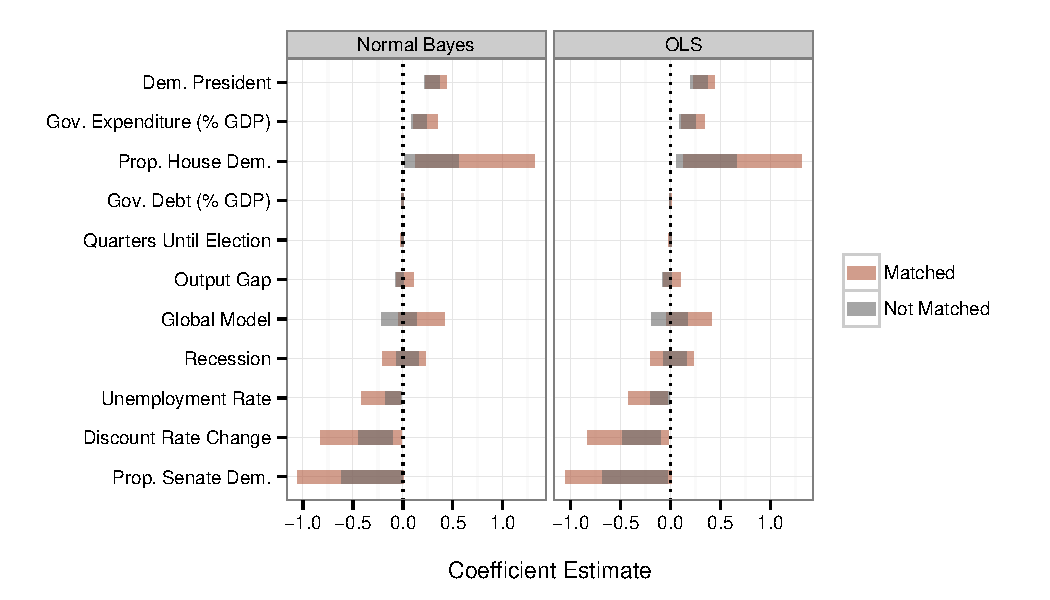
\includegraphics[width=0.95\linewidth]{figure/CoefComparePlots} 
\end{knitrout}

    \end{center}
    \begin{singlespace}
        {\scriptsize{Intercept values are not shown to maintain a reasonable scale for comparing covariate estimates.}}
    \end{singlespace}
\end{figure}

\paragraph{FRB Global Forecasting Model}

%% Check with Cassie if this Terminology is correct %%
The introduction of the FRB/Global behavioral equation forecasting model does not seem to have begun an era of significantly lower inflation forecasting error. In fact, across all of our matching and parametric model specifications, forecasts made after the introduction of this approach are not significantly different than those made before it. 

\paragraph{Presidential Elections}

We also did not find any evidence that Federal Reserve staff inflation forecast errors were associated with election timing. This was true in parametric models using both unmatched data and matched data where the election period variable is the treatment. Estimates of the relationship between the quarters until election variable and forecast errors\footnote{This variable was obviously omitted from the models with the election period variable because they are highly correlated.} also did not provide any evidence that inflation errors are related to election timing. 

Data limitations make it difficult to fully examine the extension of Clark and Arel-Bundock's \citeyearpar{Clark2011} election gaming theory for Federal Reserves staff. We only have three Democratic presidential terms in our data, only two of which ended in the incumbent running for reelection. Nonetheless, we attempted to examine this hypothesis with an interaction of the president's party ID variable and both the election dummy and quarters to election variables. In all cases the president's party ID variable was robust whereas the election variables and the interaction term were very statistically insignificant.

In this limited data set Fed Staff do not appear to be over estimating inflation when a Democratic president is running for reelection in an attempt to influence the FOMC to raise interest rates and lower the president's chances of winning. 

These findings have clear implications for how we understand the potential causes of Green Book partisan inflation forecast biases as well as FOMC interest rate decisions around elections. Federal Reserve staff do not seem to be engaged in a signalling game with the aim of influencing elections. Given both our findings and Clark and Arel-Bundock's results, it seems that FOMC members, not their staff, are driving the increases in the Fed Funds Rate around elections when Democrats are in power. 

\paragraph{Presidential Party Identification}

Our second treatment variable--presidential party identification--had a strong positive association with Federal Reserve staff inflation forecast errors across all model specifications. This finding is what we would expect if Federal Reserve staff have a general presidential partisan bias. The 95\% confidence band around the coefficient estimate actually moves somewhat further away from 0--i.e. no relationship--when using matched data (see Figure \ref{CoefComparePlots}).  

These analyses provide strong evidence that Federal Reserve staff overestimate the effect Democratic presidents have on inflation compared to Republican presidents.

\begin{figure}[t]
    \caption{Simulated Expected Inflation Forecast Error for Republican and Democratic Presidencies}
    \label{ExpectValueParty}
    \begin{center}

\begin{knitrout}
\definecolor{shadecolor}{rgb}{0.969, 0.969, 0.969}\color{fgcolor}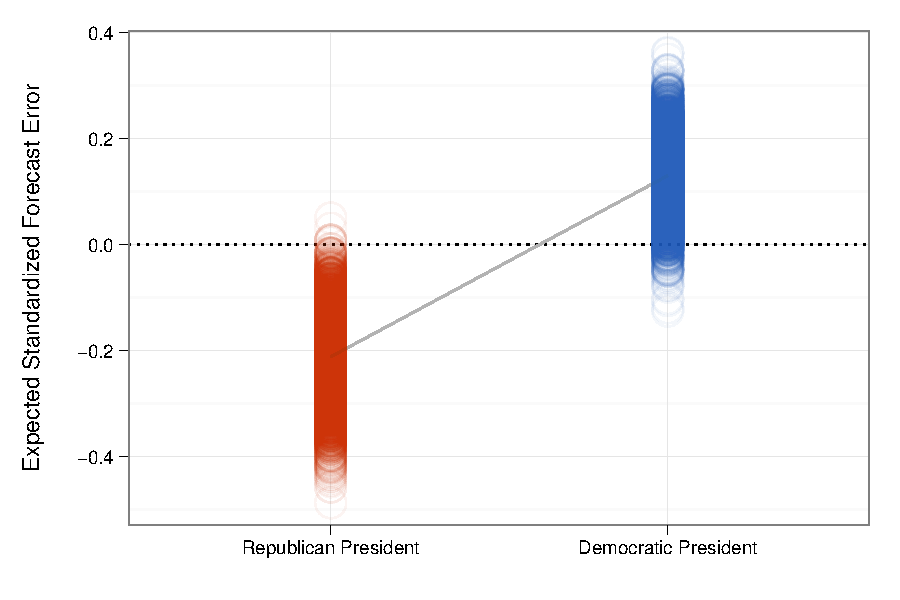
\includegraphics[width=0.7\linewidth]{figure/ExpectValueParty} 
\end{knitrout}

    \end{center}
    \begin{singlespace}
        {\scriptsize{From a normal Bayesian linear regression with data matched by presidential party identification. Variables included are the same as those in Model C6 from Table \ref{OutputPL}. The figures show 1000 simulations per fitted value. \\ The solid line connects the two groups' means.}}
    \end{singlespace}
\end{figure}

To get a sense of approximately how big this bias might be we simulated expected standardized forecast error for democratic and republican presidencies, holding all other covariates at their means.\footnote{1000 simulations were run on a normal Bayesian linear regression model matched by presidential party ID and including the same variables as those in Model C6 from Table \ref{OutputBL}.} Results from these simulations can be found in Figure \ref{ExpectValueParty}. On we expect that on average the Fed overestimates inflation by 13 percent. This compares to an average inflation error of -21 percent during Republican presidencies. Clearly, at least between 1970 and 2005, Fed staff were overly pessimistic about Democratic presidents' effect on inflation and even more overly optimistic about Republican presidents' effect. 

The estimated effects hold even when we control for actual government expenditure. This suggests that Federal Reserve staff are not simply responding to higher government expenditure that Democrats may be initiating.

\paragraph{Government Expenditure}

Nonetheless, it seems that Federal Reserve staff may also overestimate the effect of government expenditure on inflation. This is indicated by a consistently positive and significant coefficient for the government expenditure variable, even when controlling for president's party ID. Maybe Federal Reserve staff, as monetarily conservative actors, generally overestimate the effect of government expenditure on inflation.  

\paragraph{Partisan Control of Congress}

Might Federal Reserve staff be taking into consideration not only the president's party identification, but also the partisan composition of Congress? Federal Reserve staff with rational partisan expectations would presumably expect that a Democratic president would be able to get policies closer to their ideal point when there is a Congress with similar ideal preferences. If a Democratic president had chambers of Congress controlled by Democrats, presumably Federal Reserve staff would expect even higher inflation. To examine this possibility we examined models with the following interactions:

\begin{itemize}
    \item President party ID*House party ID
    \item President party ID*Senate party ID
    \item President party ID*House party ID*Senate party ID     
\end{itemize}

The interactions were generally statistically significant. To make substantive sense of these estimates we used simulations, as above, to find expected inflation forecast errors at various levels of the Presidential and Congressional party ID variables.

\begin{figure}[t]
    \caption{Simulated Interactions between President Party ID and Congressional Chamber Party Composition}
    \label{InteractionPlots}
    \begin{center}

\begin{knitrout}
\definecolor{shadecolor}{rgb}{0.969, 0.969, 0.969}\color{fgcolor}\begin{kframe}
\begin{flushleft}\ttfamily\noindent\bfseries\textcolor{errorcolor}{\#\# Error: object 'PL10.SetDem' not found}\end{flushleft}\end{kframe}
\end{knitrout}


    \end{center}
\end{figure}




\section*{Discussion: Do Fed Forecasts Have a Partisan Bias?}

FILL IN

MAYBE TALK ABOUT HOW IT IS STRANGE THAT ACTORS WITH ``RATIONAL" PARTISAN EXPECTATIONS WOULD NOT UPDATE THEIR INFLATION EXPECTATIONS. I.E. WHY WOULD THEY CONTINUE TO BE WRONG ABOUT INFLATION GIVEN THE PRESIDENT'S PARTY ID?

\clearpage
\section*{Appendix}

\subsection*{Replication}

This paper can be entirely replicated. All data, analysis source code, and markup files can be downloaded as a {\tt{.zip}} file from our GitHub page at: {\url{https://github.com/christophergandrud/GreenBook/zipball/master}}. 

{\bf{Please Note:}} This link is not currently active because we are still using a private repository to host the paper. The public repository will be available soon.

%%%%%%% Table of non-matched data with OLS parametric model %%%%%%%%

\begin{table}[ht]
    \caption{OLS Estimation of Covariate Effects on 2 Qtr. Inflation Forecast Error (non-matched dataset)}
    \label{OutputNL}
    \vspace{0.25cm}
    \begin{center}
    {\footnotesize

 
\begin{tabular}{ l D{.}{.}{1}D{.}{.}{1}D{.}{.}{1}D{.}{.}{1}D{.}{.}{1}D{.}{.}{1}D{.}{.}{1}D{.}{.}{1}D{.}{.}{1}D{.}{.}{1}D{.}{.}{1} } 
\hline 
  & \multicolumn{ 1 }{ c }{ A1 } & \multicolumn{ 1 }{ c }{ A2 } & \multicolumn{ 1 }{ c }{ A3 } & \multicolumn{ 1 }{ c }{ A4 } & \multicolumn{ 1 }{ c }{ A5 } & \multicolumn{ 1 }{ c }{ A6 } & \multicolumn{ 1 }{ c }{ A7 } & \multicolumn{ 1 }{ c }{ A8 } & \multicolumn{ 1 }{ c }{ A9 } & \multicolumn{ 1 }{ c }{ A10 } & \multicolumn{ 1 }{ c }{ A11 } \\ \hline
 %                    & A1             & A2             & A3             & A4             & A5             & A6             & A7             & A8             & A9             & A10            & A11           \\ 
Intercept            & 3.2 ^{**}      & 3.4 ^{**}      & 3.2 ^{**}      & 3.3 ^{***}     & 3.6 ^{***}     & 3.8 ^{***}     & 3.7 ^{***}     & 3.6 ^{***}     & 3.2 ^{***}     & 1.3            & -2.2 ^{***}   \\ 
                     & (1.1)          & (1.1)          & (1.1)          & (0.9)          & (0.9)          & (0.9)          & (0.9)          & (0.9)          & (0.9)          & (1.2)          & (0.4)         \\ 
Recession            & -0.0           & 0.0            & -0.0           & 0.1            & 0.1            & 0.1            & 0.1            & 0.1 ^*         & 0.1 ^\dagger  & 0.1            &               \\ 
                     & (0.1)          & (0.1)          & (0.1)          & (0.1)          & (0.1)          & (0.1)          & (0.1)          & (0.0)          & (0.0)          & (0.0)          &               \\ 
Debt/GDP             & 0.0            & 0.0            & 0.0            & -0.0           & -0.0           & 0.0            & 0.0            & -0.0           & -0.0           & 0.0            &               \\ 
                     & (0.0)          & (0.0)          & (0.0)          & (0.0)          & (0.0)          & (0.0)          & (0.0)          & (0.0)          & (0.0)          & (0.0)          &               \\ 
Expenditure/GDP      & 0.1 ^{***}     & 0.1 ^{***}     & 0.1 ^{***}     & 0.2 ^{***}     & 0.2 ^{***}     & 0.1 ^{***}     & 0.1 ^{**}      & 0.1 ^{***}     & 0.1 ^{***}     & 0.1 ^{**}      &               \\ 
                     & (0.0)          & (0.0)          & (0.0)          & (0.0)          & (0.0)          & (0.0)          & (0.0)          & (0.0)          & (0.0)          & (0.0)          &               \\ 
Output Gap           & -0.1 ^{***}    & -0.1 ^{***}    & -0.1 ^{***}    & -0.1 ^{***}    & -0.1 ^{***}    & -0.1 ^{***}    & -0.1 ^{***}    & -0.1 ^{***}    & -0.1 ^{***}    & -0.1 ^{***}    &               \\ 
                     & (0.0)          & (0.0)          & (0.0)          & (0.0)          & (0.0)          & (0.0)          & (0.0)          & (0.0)          & (0.0)          & (0.0)          &               \\ 
Qtr. to Election     &                & -0.0           &                &                & -0.0           & -0.0           & -0.0           & 0.0            & 0.0            & 0.0            &               \\ 
                     &                & (0.0)          &                &                & (0.0)          & (0.0)          & (0.0)          & (0.0)          & (0.0)          & (0.0)          &               \\ 
Election Period      &                &                & 0.0            &                &                &                &                &                &                &                &               \\ 
                     &                &                & (0.1)          &                &                &                &                &                &                &                &               \\ 
Pres. Party ID       &                &                &                & 0.3 ^{***}     & 0.3 ^{***}     & 0.3 ^{***}     & 0.3 ^{***}     & 0.9 ^{***}     & 1.1 ^{***}     & 2.4 ^{***}     & 2.6 ^{***}    \\ 
                     &                &                &                & (0.0)          & (0.0)          & (0.0)          & (0.0)          & (0.1)          & (0.2)          & (0.7)          & (0.7)         \\ 
Senate Dem/Rep       &                &                &                &                &                & -0.2           & -0.3           & -0.2           & -0.0           & 0.9 ^*         & 1.1 ^{***}    \\ 
                     &                &                &                &                &                & (0.1)          & (0.2)          & (0.1)          & (0.1)          & (0.3)          & (0.3)         \\ 
House Dem/Rep        &                &                &                &                &                & 0.2            & 0.2            & 0.4 ^{***}     & 0.3 ^{**}      & 1.3 ^{***}     & 1.8 ^{***}    \\ 
                     &                &                &                &                &                & (0.1)          & (0.1)          & (0.1)          & (0.1)          & (0.3)          & (0.3)         \\ 
FRB/GlobalModel      &                &                &                &                &                &                & -0.1           &                &                &                &               \\ 
                     &                &                &                &                &                &                & (0.1)          &                &                &                &               \\ 
Pres Party ID*House  &                &                &                &                &                &                &                & -0.5 ^{***}    &                & -1.8 ^*        & -2.6 ^{**}    \\ 
                     &                &                &                &                &                &                &                & (0.1)          &                & (0.8)          & (0.8)         \\ 
Pres Party ID*Senate &                &                &                &                &                &                &                &                & -0.7 ^{***}    & -1.1           & -0.6          \\ 
                     &                &                &                &                &                &                &                &                & (0.1)          & (0.7)          & (0.6)         \\ 
House*Senate         &                &                &                &                &                &                &                &                &                & -0.7 ^{**}     & -1.0 ^{***}   \\ 
                     &                &                &                &                &                &                &                &                &                & (0.2)          & (0.2)         \\ 
Pres*House*Senate    &                &                &                &                &                &                &                &                &                & 0.9 ^*         & 1.2 ^*        \\ 
                     &                &                &                &                &                &                &                &                &                & (0.4)          & (0.5)          \\
 $N$                  & 148            & 148            & 148            & 148            & 148            & 148            & 148            & 148            & 148            & 148            & 148           \\ 
$R^2$                & 0.3            & 0.3            & 0.3            & 0.5            & 0.5            & 0.5            & 0.5            & 0.6            & 0.6            & 0.6            & 0.5           \\ 
adj. $R^2$           & 0.3            & 0.3            & 0.2            & 0.5            & 0.5            & 0.5            & 0.5            & 0.6            & 0.5            & 0.6            & 0.5           \\ 
Resid. sd            & 0.2            & 0.2            & 0.2            & 0.2            & 0.2            & 0.2            & 0.2            & 0.2            & 0.2            & 0.2            & 0.2            \\ \hline
 \multicolumn{12}{l}{\footnotesize{Standard errors in parentheses}}\\
\multicolumn{12}{l}{\footnotesize{$^\dagger$ significant at $p<.10$; $^* p<.05$; $^{**} p<.01$; $^{***} p<.001$}} 
\end{tabular} 



    }
    \end{center}
\end{table}

%%%%%%% Table of ElectionPeriod matched data with OLS parametric model %%%%%%%%

\begin{table}[ht]
    \caption{OLS Estimation of Covariate Effects on 2 Qtr. Inflation Forecast Error (Matched by Election Period Variable)}
    \label{OutputEL}
    \vspace{0.25cm}
    \begin{center}
    {\footnotesize

 
\begin{tabular}{ l D{.}{.}{1}D{.}{.}{1}D{.}{.}{1}D{.}{.}{1}D{.}{.}{1}D{.}{.}{1}D{.}{.}{1}D{.}{.}{1}D{.}{.}{1}D{.}{.}{1}D{.}{.}{1} } 
\hline 
  & \multicolumn{ 1 }{ c }{ B1 } & \multicolumn{ 1 }{ c }{ B2 } & \multicolumn{ 1 }{ c }{ B3 } & \multicolumn{ 1 }{ c }{ B4 } & \multicolumn{ 1 }{ c }{ B5 } & \multicolumn{ 1 }{ c }{ B6 } & \multicolumn{ 1 }{ c }{ B7 } & \multicolumn{ 1 }{ c }{ B8 } & \multicolumn{ 1 }{ c }{ B9 } & \multicolumn{ 1 }{ c }{ B10 } & \multicolumn{ 1 }{ c }{ B11 } \\ \hline
 %                    & B1              & B2              & B3              & B4              & B5              & B6              & B7              & B8              & B9              & B10             & B11            \\ 
Intercept            & -1.0            & -0.8            & -1.0            & 1.3             & 1.5             & 4.0             & 3.1             & 2.6             & 1.5             & 1.6             & -3.5 ^{***}    \\ 
                     & (4.0)           & (4.1)           & (4.0)           & (3.2)           & (3.2)           & (3.6)           & (5.0)           & (2.7)           & (3.0)           & (4.4)           & (0.9)          \\ 
Debt/GDP             & -0.0            & -0.0            & -0.0            & -0.0            & -0.0            & 0.0             & 0.0             & -0.0            & -0.0            & 0.0             &                \\ 
                     & (0.0)           & (0.0)           & (0.0)           & (0.0)           & (0.0)           & (0.0)           & (0.0)           & (0.0)           & (0.0)           & (0.0)           &                \\ 
Expenditure/GDP      & 0.1 ^*          & 0.2 ^*          & 0.1 ^*          & 0.2 ^{***}      & 0.2 ^{***}      & 0.2 ^*          & 0.2             & 0.3 ^{***}      & 0.3 ^{***}      & -0.0            &                \\ 
                     & (0.1)           & (0.1)           & (0.1)           & (0.1)           & (0.1)           & (0.1)           & (0.1)           & (0.1)           & (0.1)           & (0.1)           &                \\ 
Output Gap           & -0.0            & -0.0            & -0.0            & -0.1            & -0.1            & -0.1 ^\dagger  & -0.1            & -0.1 ^*         & -0.1 ^*         & -0.1            &                \\ 
                     & (0.0)           & (0.0)           & (0.0)           & (0.0)           & (0.0)           & (0.0)           & (0.1)           & (0.0)           & (0.0)           & (0.0)           &                \\ 
Qtr. to Election     &                 & 0.0             &                 &                 & 0.0             & 0.0             & 0.0             & 0.0             & 0.0             & 0.0             &                \\ 
                     &                 & (0.0)           &                 &                 & (0.0)           & (0.0)           & (0.0)           & (0.0)           & (0.0)           & (0.0)           &                \\ 
Election Period      &                 &                 & 0.1             &                 &                 &                 &                 &                 &                 &                 &                \\ 
                     &                 &                 & (0.1)           &                 &                 &                 &                 &                 &                 &                 &                \\ 
Pres. Party ID       &                 &                 &                 & 0.4 ^{***}      & 0.4 ^{***}      & 0.5 ^{***}      & 0.5 ^{***}      & 1.5 ^{***}      & 1.9 ^{***}      & 0.1             & 0.8 ^\dagger  \\ 
                     &                 &                 &                 & (0.1)           & (0.1)           & (0.1)           & (0.1)           & (0.3)           & (0.4)           & (0.7)           & (0.4)          \\ 
Senate Dem/Rep       &                 &                 &                 &                 &                 & 0.1             & 0.0             & 0.4             & 0.5             & 1.2             & 2.0 ^*         \\ 
                     &                 &                 &                 &                 &                 & (0.4)           & (0.4)           & (0.3)           & (0.3)           & (1.1)           & (0.8)          \\ 
House Dem/Rep        &                 &                 &                 &                 &                 & 0.4             & 0.3             & 0.2             & -0.0            & 2.5 ^*          & 2.4 ^{***}     \\ 
                     &                 &                 &                 &                 &                 & (0.4)           & (0.4)           & (0.3)           & (0.3)           & (1.0)           & (0.5)          \\ 
FRB/GlobalModel      &                 &                 &                 &                 &                 &                 & -0.1            &                 &                 &                 &                \\ 
                     &                 &                 &                 &                 &                 &                 & (0.4)           &                 &                 &                 &                \\ 
Pres Party ID*House  &                 &                 &                 &                 &                 &                 &                 & -0.9 ^{***}     &                 & -3.6 ^{**}      & -3.1 ^{***}    \\ 
                     &                 &                 &                 &                 &                 &                 &                 & (0.2)           &                 & (1.0)           & (0.6)          \\ 
Pres Party ID*Senate &                 &                 &                 &                 &                 &                 &                 &                 & -1.3 ^{**}      & 4.5 ^*          & 3.3 ^{**}      \\ 
                     &                 &                 &                 &                 &                 &                 &                 &                 & (0.4)           & (1.7)           & (0.9)          \\ 
House*Senate         &                 &                 &                 &                 &                 &                 &                 &                 &                 & -1.0            & -1.4 ^{**}     \\ 
                     &                 &                 &                 &                 &                 &                 &                 &                 &                 & (0.7)           & (0.4)           \\
 $N$                  & 30              & 30              & 30              & 30              & 30              & 30              & 30              & 30              & 30              & 30              & 30             \\ 
$R^2$                & 0.2             & 0.3             & 0.3             & 0.6             & 0.6             & 0.6             & 0.6             & 0.8             & 0.8             & 0.9             & 0.8            \\ 
adj. $R^2$           & 0.2             & 0.1             & 0.1             & 0.5             & 0.5             & 0.5             & 0.5             & 0.7             & 0.7             & 0.8             & 0.8            \\ 
Resid. sd            & 0.3             & 0.3             & 0.3             & 0.2             & 0.2             & 0.2             & 0.2             & 0.2             & 0.2             & 0.1             & 0.2             \\ \hline
 \multicolumn{12}{l}{\footnotesize{Standard errors in parentheses}}\\
\multicolumn{12}{l}{\footnotesize{$^\dagger$ significant at $p<.10$; $^* p<.05$; $^{**} p<.01$; $^{***} p<.001$}}\\
\multicolumn{12}{l}{\footnotesize{The recession variable is ommitted because there was no variation in the matched data set.}}\\
\multicolumn{12}{l}{\footnotesize{The reason that there was no variation is because there was never a recession during an}}\\
\multicolumn{12}{l}{\footnotesize{election period in our data set.}} 
\end{tabular} 



    }
    \end{center}
\end{table}

%%%%%%% Table of pres_party matched data with OLS parametric model %%%%%%%%

\begin{table}[ht]
    \caption{OLS Estimation of Covariate Effects on 2 Qtr. Inflation Forecast Error (Matched by President's Party ID variable)}
    \label{OutputPL}
    \vspace{0.25cm}
    \begin{center}
    {\footnotesize

 
\begin{tabular}{ l D{.}{.}{1}D{.}{.}{1}D{.}{.}{1}D{.}{.}{1}D{.}{.}{1}D{.}{.}{1}D{.}{.}{1}D{.}{.}{1}D{.}{.}{1}D{.}{.}{1}D{.}{.}{1} } 
\hline 
  & \multicolumn{ 1 }{ c }{ C1 } & \multicolumn{ 1 }{ c }{ C2 } & \multicolumn{ 1 }{ c }{ C3 } & \multicolumn{ 1 }{ c }{ C4 } & \multicolumn{ 1 }{ c }{ C5 } & \multicolumn{ 1 }{ c }{ C6 } & \multicolumn{ 1 }{ c }{ C7 } & \multicolumn{ 1 }{ c }{ C8 } & \multicolumn{ 1 }{ c }{ C9 } & \multicolumn{ 1 }{ c }{ C10 } & \multicolumn{ 1 }{ c }{ C11 } \\ \hline
 %                    & C1              & C2              & C3              & C4              & C5              & C6              & C7              & C8              & C9              & C10             & C11            \\ 
Intercept            & 2.4             & 2.4             & 2.6             & 1.1             & 1.1             & -0.8            & -0.8            & 0.4             & 0.1             & -2.7            & -2.1 ^{***}    \\ 
                     & (2.7)           & (2.8)           & (2.8)           & (2.2)           & (2.2)           & (2.4)           & (2.4)           & (2.0)           & (2.0)           & (2.4)           & (0.6)          \\ 
Recession            & 0.1             & 0.1             & 0.1             & 0.1             & 0.1             & 0.1             & 0.1             & 0.1             & 0.1             & 0.0             &                \\ 
                     & (0.2)           & (0.2)           & (0.2)           & (0.1)           & (0.1)           & (0.1)           & (0.1)           & (0.1)           & (0.1)           & (0.1)           &                \\ 
Debt/GDP             & 0.0             & 0.0             & 0.0             & 0.0             & 0.0             & -0.0            & -0.0            & -0.0            & -0.0            & -0.0            &                \\ 
                     & (0.0)           & (0.0)           & (0.0)           & (0.0)           & (0.0)           & (0.0)           & (0.0)           & (0.0)           & (0.0)           & (0.0)           &                \\ 
Expenditure/GDP      & 0.1 ^*          & 0.1 ^*          & 0.1 ^*          & 0.1 ^*          & 0.1 ^*          & 0.1 ^\dagger   & 0.1             & 0.1 ^*          & 0.1 ^{**}       & 0.0             &                \\ 
                     & (0.1)           & (0.1)           & (0.1)           & (0.0)           & (0.0)           & (0.1)           & (0.1)           & (0.0)           & (0.0)           & (0.1)           &                \\ 
Output Gap           & -0.0            & -0.0            & -0.1            & -0.0            & -0.0            & -0.0            & -0.0            & -0.0            & -0.0            & -0.0            &                \\ 
                     & (0.0)           & (0.0)           & (0.0)           & (0.0)           & (0.0)           & (0.0)           & (0.0)           & (0.0)           & (0.0)           & (0.0)           &                \\ 
Qtr. to Election     &                 & -0.0            &                 &                 & -0.0            & -0.0            & -0.0            & 0.0             & 0.0             & 0.0             &                \\ 
                     &                 & (0.0)           &                 &                 & (0.0)           & (0.0)           & (0.0)           & (0.0)           & (0.0)           & (0.0)           &                \\ 
Election Period      &                 &                 & -0.1            &                 &                 &                 &                 &                 &                 &                 &                \\ 
                     &                 &                 & (0.1)           &                 &                 &                 &                 &                 &                 &                 &                \\ 
Pres. Party ID       &                 &                 &                 & 0.3 ^{***}      & 0.3 ^{***}      & 0.3 ^{***}      & 0.3 ^{***}      & 1.2 ^{***}      & 1.4 ^{***}      & 2.7 ^{**}       & 2.6 ^{**}      \\ 
                     &                 &                 &                 & (0.1)           & (0.1)           & (0.1)           & (0.1)           & (0.2)           & (0.2)           & (0.9)           & (0.8)          \\ 
Senate Dem/Rep       &                 &                 &                 &                 &                 & -0.8 ^*         & -0.8 ^\dagger  & -0.4            & -0.1            & 0.6             & 0.5            \\ 
                     &                 &                 &                 &                 &                 & (0.4)           & (0.4)           & (0.3)           & (0.3)           & (0.7)           & (0.6)          \\ 
House Dem/Rep        &                 &                 &                 &                 &                 & 0.4             & 0.4             & 0.6 ^*          & 0.4 ^\dagger   & 2.1 ^{**}       & 2.4 ^{***}     \\ 
                     &                 &                 &                 &                 &                 & (0.3)           & (0.3)           & (0.2)           & (0.2)           & (0.7)           & (0.5)          \\ 
FRB/GlobalModel      &                 &                 &                 &                 &                 &                 & -0.0            &                 &                 &                 &                \\ 
                     &                 &                 &                 &                 &                 &                 & (0.1)           &                 &                 &                 &                \\ 
Pres Party ID*House  &                 &                 &                 &                 &                 &                 &                 & -0.7 ^{***}     &                 & -2.7 ^*         & -3.2 ^{***}    \\ 
                     &                 &                 &                 &                 &                 &                 &                 & (0.1)           &                 & (1.1)           & (0.9)          \\ 
Pres Party ID*Senate &                 &                 &                 &                 &                 &                 &                 &                 & -0.9 ^{***}     & -0.6            & 0.0            \\ 
                     &                 &                 &                 &                 &                 &                 &                 &                 & (0.2)           & (1.2)           & (0.8)          \\ 
House*Senate         &                 &                 &                 &                 &                 &                 &                 &                 &                 & -1.0 ^*         & -1.1 ^{**}     \\ 
                     &                 &                 &                 &                 &                 &                 &                 &                 &                 & (0.4)           & (0.4)          \\ 
Pres*House*Senate    &                 &                 &                 &                 &                 &                 &                 &                 &                 & 1.2 ^*          & 1.2 ^*         \\ 
                     &                 &                 &                 &                 &                 &                 &                 &                 &                 & (0.6)           & (0.5)           \\
 $N$                  & 70              & 70              & 70              & 70              & 70              & 70              & 70              & 70              & 70              & 70              & 70             \\ 
$R^2$                & 0.1             & 0.1             & 0.1             & 0.4             & 0.4             & 0.5             & 0.5             & 0.6             & 0.6             & 0.7             & 0.7            \\ 
adj. $R^2$           & 0.1             & 0.0             & 0.1             & 0.4             & 0.4             & 0.4             & 0.4             & 0.6             & 0.6             & 0.6             & 0.6            \\ 
Resid. sd            & 0.3             & 0.3             & 0.3             & 0.2             & 0.2             & 0.2             & 0.2             & 0.2             & 0.2             & 0.2             & 0.2             \\ \hline
 \multicolumn{12}{l}{\footnotesize{Standard errors in parentheses}}\\
\multicolumn{12}{l}{\footnotesize{$^\dagger$ significant at $p<.10$; $^* p<.05$; $^{**} p<.01$; $^{***} p<.001$}} 
\end{tabular} 



    }
    \end{center}
\end{table}

%%%%%%% Table of pres_party matched data with Bayesian normal linear parametric 

% latex table generated in R 2.15.1 by xtable 1.7-0 package
% Thu Jul 19 17:00:53 2012
\begin{table}[ht]
\begin{center}
\caption{Bayesian Normal Linear Regression Estimation of Covariate Effects on 2 Qtr. Inflation Forecast Error (non-matched data set)}
\label{OutputNB}
{\small
\begin{tabular}{lccccc}
  \hline
Variables & Mean & SD & 2.5\% & 50\% & 97.5\% \\ 
  \hline
Intercept & 3.71 & 0.95 & 1.87 & 3.71 & 5.59 \\ 
  Pres. Party ID & 0.25 & 0.04 & 0.18 & 0.25 & 0.33 \\ 
  Recession & 0.08 & 0.05 & -0.02 & 0.08 & 0.19 \\ 
  Qtr. to Election & -0.00 & 0.00 & -0.01 & -0.00 & 0.00 \\ 
  Senate Dem/Rep & -0.26 & 0.16 & -0.56 & -0.25 & 0.06 \\ 
  House Dem/Rep & 0.20 & 0.13 & -0.05 & 0.20 & 0.46 \\ 
  Debt/GDP & 0.00 & 0.00 & -0.00 & 0.00 & 0.01 \\ 
  Expenditure/GDP & 0.12 & 0.04 & 0.05 & 0.12 & 0.19 \\ 
  Output Gap & -0.06 & 0.01 & -0.09 & -0.06 & -0.04 \\ 
  Global Model & -0.06 & 0.08 & -0.23 & -0.06 & 0.10 \\ 
  sigma2 & 0.04 & 0.00 & 0.03 & 0.04 & 0.05 \\ 
   \hline
\end{tabular}
}
\end{center}
\end{table}





%%%%%%% Table of pres_party matched data with Normal Bayesian linear parametric model %%%%%%%%


% latex table generated in R 2.15.1 by xtable 1.7-0 package
% Thu Jul 19 17:00:54 2012
\begin{table}[ht]
\begin{center}
\caption{Bayesian Normal Linear Regression Estimation of Covariate Effects on 2 Qtr. Inflation Forecast Error (Matched by President's Party ID variable}
\label{OutputPB}
{\small
\begin{tabular}{lccccc}
  \hline
Variables & Mean & SD & 2.5\% & 50\% & 97.5\% \\ 
  \hline
Intercept & -0.84 & 2.44 & -5.58 & -0.85 & 4.00 \\ 
  Pres. Party ID & 0.34 & 0.06 & 0.22 & 0.34 & 0.46 \\ 
  Recession & 0.08 & 0.13 & -0.17 & 0.08 & 0.33 \\ 
  Qtr. to Election & -0.00 & 0.01 & -0.01 & -0.00 & 0.01 \\ 
  Senate Dem/Rep & -0.76 & 0.41 & -1.56 & -0.77 & 0.04 \\ 
  House Dem/Rep & 0.42 & 0.29 & -0.15 & 0.42 & 0.98 \\ 
  Debt/GDP & -0.00 & 0.01 & -0.01 & -0.00 & 0.01 \\ 
  Expenditure/GDP & 0.10 & 0.07 & -0.03 & 0.10 & 0.24 \\ 
  Output Gap & -0.01 & 0.03 & -0.08 & -0.01 & 0.05 \\ 
  Global Model & -0.01 & 0.12 & -0.24 & -0.01 & 0.23 \\ 
  sigma2 & 0.05 & 0.01 & 0.03 & 0.05 & 0.07 \\ 
   \hline
\end{tabular}
}
\end{center}
\end{table}




%%%%%%% References %%%%%%%%%%%%

\clearpage

\bibliographystyle{apsr}
\bibliography{GreenBook.bib}

\end{document}
